\documentclass[paper=letter, fontsize=11pt]{scrartcl} 
\usepackage{graphicx}
\usepackage{verbatim}
\usepackage{pictex}  
\usepackage{multimedia}
\usepackage{listings}
\usepackage{xcolor,colortbl}
\usepackage[utf8]{inputenc}		%para identificar acentos(encoding)
\usepackage{url}
\usepackage[spanish]{babel} % language/hyphenation
\usepackage{amsmath,amsfonts,amsthm} % Math packages
\usepackage{amsbsy}
\usepackage{amssymb}
\usepackage{fancyvrb}
\usepackage{sectsty} % Allows customizing section commands
\setcounter{section}{-1}
\allsectionsfont{\centering \normalfont\scshape} % Make all sections centered, the default font and small caps
\usepackage{float}%para fijar las figuras y tablas
\usepackage{placeins}%fija espacios
\usepackage{fancyhdr} % Custom headers and footers
\pagestyle{fancyplain} % Makes all pages in the document conform to the custom headers and footers
\fancyhead{} % No page header - if you want one, create it in the same way as the footers below
\fancyfoot[L]{} % Empty left footer
\fancyfoot[C]{} % Empty center footer
\fancyfoot[R]{\thepage} % Page numbering for right footer
\renewcommand{\headrulewidth}{0pt} % Remove header underlines
\renewcommand{\footrulewidth}{0pt} % Remove footer underlines
\setlength{\headheight}{2.6pt} % Customize the height of the header

\numberwithin{equation}{section} % Number equations within sections (i.e. 1.1, 1.2, 2.1, 2.2 instead of 1, 2, 3, 4)
\numberwithin{figure}{section} % Number figures within sections (i.e. 1.1, 1.2, 2.1, 2.2 instead of 1, 2, 3, 4)
\numberwithin{table}{section} % Number tables within sections (i.e. 1.1, 1.2, 2.1, 2.2 instead of 1, 2, 3, 4)

\setlength\parindent{0pt} % Removes all indentation from paragraphs - comment this line for an assignment with lots of text

\newcommand{\horrule}[1]{\rule{\linewidth}{#1}} % Create horizontal rule command with 1 argument of height

\title{	
\normalfont \normalsize 
\textsc{Centro de Investigaci\'on en Matem\'aticas (CIMAT). Unidad Monterrey.} 
\\ [25pt] 
\horrule{0.5pt} \\[0.1cm] % Thin top horizontal rule
\Large La encuesta de habilidades de CONOCER (2012) vista en bajas dimensiones. \\ 
\small Una aplicación de MDS unfolding
\horrule{0.5pt} \\[0.1cm] % Thick bottom horizontal rule
}

\author{José Antonio Garcia Ramirez} % Your name

\date{\normalsize\today} % Today's date or a custom date

\begin{document}
\lstdefinestyle{customc}{
  belowcaptionskip=1\baselineskip,
  basicstyle=\footnotesize, 
  frame=lrtb,
  breaklines=true,
  %frame=L,
  %xleftmargin=\parindent,
  language=C,
  showstringspaces=false,
  basicstyle=\footnotesize\ttfamily,
  keywordstyle=\bfseries\color{green!40!black},
  commentstyle=\itshape\color{red!40!black},
  identifierstyle=\color{blue},
  stringstyle=\color{purple},
}

\lstset{breakatwhitespace=true,
  basicstyle=\footnotesize, 
  commentstyle=\color{green},
  keywordstyle=\color{blue},
  stringstyle=\color{purple},
  language=C++,
  columns=fullflexible,
  keepspaces=true,
  breaklines=true,
  tabsize=3, 
  showstringspaces=false,
  extendedchars=true}

\lstset{ %
  language=R,    
  basicstyle=\footnotesize, 
  numbers=left,             
  numberstyle=\tiny\color{gray}, 
  stepnumber=1,              
  numbersep=5pt,             
  backgroundcolor=\color{white},
  showspaces=false,             
  showstringspaces=false,       
  showtabs=false,               
  frame=single,                 
  rulecolor=\color{black},      
  tabsize=2,                  
  captionpos=b,               
  breaklines=true,            
  breakatwhitespace=false,    
  title=\lstname,             
  keywordstyle=\color{blue},  
  commentstyle=\color{dkgreen},
  stringstyle=\color{mauve},   
  morekeywords={\%*\%,...}         
} 


\maketitle % Print the title

\section{Antecedentes: Sobre la encuesta de habilidades de CONOCER del 2012}
El Consejo Nacional de Normalización y Certificación de Competencias Laborales, CONOCER, quien coordina y promueve el Sistema Nacional de Competencias, para que México cuente con empresarios, trabajadores, docentes, estudiantes y servidores públicos más competentes realizó en el 2012 un estudio para fortalecer la estrategia de promoción y desarrollo del Sistema Nacional de Competencias con relación a competencias de personas y perfiles ocupacionales en México.\\
Algunos de los objetivos de tal estudio fueron:
\begin{itemize}
\item Obtener información respecto a las competencias requeridas para las ocupaciones en México. Construyendo una encuesta que fue aplicada a 18,000 empresarios y trabajadores del país.

\item Identificar a nivel macro las necesidades sectoriales\footnote{En el sentido de sectores económicos, no sectores demográficos propiamente.} existentes.

\item Detectar competencias transversales es decir aquellas que su prevalencia y su efecto en una muestra poblacional en un solo momento temporal favorezca a la industria y gobierno.

\item Contar con información adicional, para apoyar la pertinencia de la oferta educativa a los requerimientos de la demanda laboral.
\end{itemize}
El estudio se basó en el Sistema Nacional de Clasificación de Ocupaciones (SINCO) que es una documento de consulta para clasificar, ordenar y describir las ocupaciones que se realizan en el país\footnote{ Para más detalles del SINCO puede consultarse el Diario Oficial de la Federación del 12 de abril de 2012 en su sitio web.}.\\

\subsection{Objetivo}

En el presente documento exploramos la encuesta de habilidades que contiene una mezcla de técnicas cualitativas y cuantitativas Con el objetivo primario de explorar la asociación entre habilidades que aborda la encuesta de CONOCER sobre el conjunto de ocupaciones que la misma contempla, en segundo lugar se busca verificar (y en medida de lo posible ampliar) los resultados obtenidos en este trabajo y los que se mencionaron en la plática del Dr. Miguel Flores en el seminario de CIMAT unidad Monterrey el 15 de marzo de 2018.


\subsection{El cuestionario }

A raíz de una charla que el Dr. Miguel Flores presentó en CIMAT unidad monterrey el pasado 15 de marzo, donde se habló de sueldos, salarios y la distribución geográfica de competencias en el país para prever y realizar las políticas públicas que beneficien al bien común. \\

Al final de las charla el Dr. Miguel Ángel mostró apertura a compartir los datos de la encuesta de habilidades, que fue parte importante de su estudio. Por lo que accedimos y realizamos la petición de los datos.   \\

Respecto a los datos proporcionados y a la encuesta-entrevista se definió lo siguiente: La unidad de observación son los centros de trabajo, la unidad de análisis son los empleados o directivos con al menos un año de experiencia en su respectiva ocupación (se planeó que los 445 grupos unitarios del SINCO estuviesen presentes). El método de aplicación consistió en entrevista directa en el lugar de trabajo. El cuestionario es semiestructurado pues contiene 150 preguntas de las cuales el 90\% son cerradas. \\

El cuestionario (que anexamos en el archivo ‘Cuest\_Conocer\_2011\_Ok-REV 04-03-2011.doc’) se integra por dos partes, la primera la contesta el patrón o supervisor directo del trabajador encuestado, esto con la finalidad de captar información sobre las características cualitativas del centro de trabajo. La segunda sección se centró en captar los rasgos cualitativos de los grupos unitarios  \\

La mayor parte de las preguntas (102 para ser exactos) son cerradas y corresponden a variables ordinarias en una escala de 1 a 5 (donde 5 expresa que 	 	 	
el mismo trabajador determinó que es muy relevante el rasgo para definir el perfil de su puesto de trabajo  y 1 en el caso opuesto, esto nos permitió considerar en el análisis exploratorio el modelo de escalamiento multidimensional de despliegue, MDS unfolding).\\

El resto de las preguntas, algunas cerradas y otras abiertas, contienen texto que como veremos en la siguiente sección nos permitió identificar la distribución espacial de los empleados y algunas otras características. \\

Los criterios para elegir a las empresas donde se realizaron las entrevistas se consideraron por cada grupo unitario los subsectores de actividad económica en donde se tiene la mayor parte de los ocupados (según el Sistema de Clasificación Industrial de América del Norte). La cota superior fue de entrevistar a lo más tres trabajadores por empresa.
\section{Metodología}
\subsection{Obtención de los datos}
Si bien el Dr. Miguel Flores nos proporciono un archivo .xlsx semiestructurado con 17,250 observaciones que corresponden a entrevistas campatadas en 13,250 centros labolares (en nuestro conjunto de datos se cuentan 14498 empresas sin embargo esto se debe a errores de captura pues en algunos casos el nombre de la empresa fue capturado con variaciones de puntos, letras, comas o espacios de más) a trabajadores con al menos un año de experiencia en su ocupación, fue necesario consultar en el sitio web del INEGI relativo al SINCO \url{http://www3.inegi.org.mx/sistemas/clasificaciones/sinco/sinco.aspx} para obtener las descripciones de las ocupaciones de las que solo se nos proporcionaron los identificadores de 4 digitos \footnote{ Este procedimiento tiene que ser manual con la actual implementación del sitio web, lo cual fue demandante en tiempo y cuyo resultado se encuentra en el archivo anexo ‘A.csv’ } adémas para lograr una identificación más sencilla de las actividades empresariales y brindar mayor claridad al análisis descriptivo de algunas de las variables se capturaron manualmente las descripciones de varias variables de las que igualmente solo se disponia de una clave y no de la descripción (el codigo anexo ‘Conocer.R’ refleja este trabajo).\\

En vista de lo costoso que resulta este esquema de la encuesta de habilidades (pues es en principio es un muestreo complejo) y requiere de un costo de implementación elevado, la encuesta no se ha vuelto a repetir, sin embargo son datos que encajan bien con el modelo MDS unfolding (ya que de entrada son disimilaridades y permitirán validar o rechazar conjeturas sobre los grupos).

\subsection{Análisis de la encuesta de habilidades}
Considerando la dimensionalidad el conjunto de datos con el que estamos trabajando, 150 variables y un número de muestra de 17,250. Y aprovechando el hecho de que la encuesta se compone de dos etapas, comenzamos con un análisis descriptivo y espacial sobre algunas variables y procedemos después con una exploración a intentar identificar grupos de puestos de trabajo o bien grupos de habilidades que sean comunes. Para ello utilizamos el enfoque de MDS unfolding pues los datos que tenemos representan ciertamente proximidades entre dos modos (los empleados y las habilidades). El reto es que todas las variables que tienen la misma escala y reflejan las proximidades son ordinarias, por lo cual de acuerdoa a \cite{roris} son computacionalmente intensivos aún utilizando el algoritmo de SMACOF implementado en R\cite{R} basado en el trabajo \cite{smacof} en el paquete SMACOF de R\cite{Rsmacof}.\\

En la figura 1.1 mostramos dos mapas, donde los estados con colores más saturados corresponden a estados con mayor participación de empresas (derecha) y de empleados (izquierda) por estado dentro de la muestra. Es de esperarse que estos mapas sean parecidos pero no idénticos ya que como se mencionó el criterio de elección de las empresas fue el de pertenecer al subsector económico con mayor número de empleados contratados en un determinado grupo. 
\begin{figure}[H]
  \begin{center}
    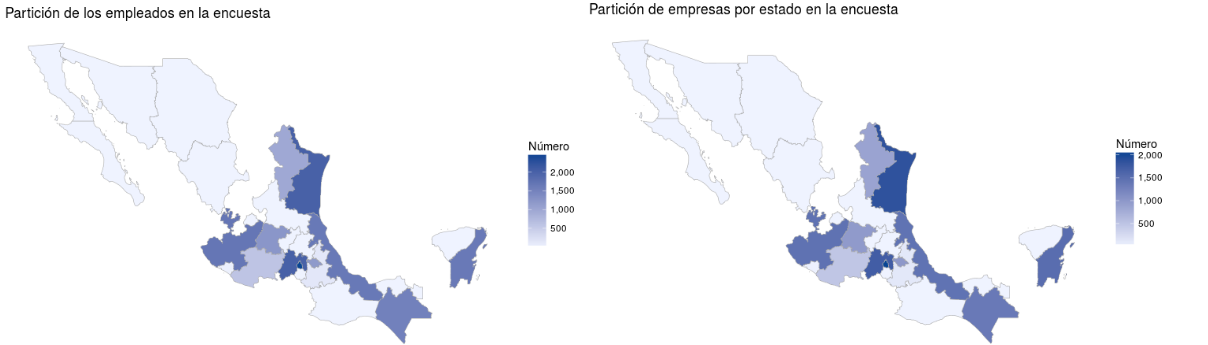
\includegraphics[scale=.4]{mapas.png}
    \caption{Distribución geográfica por entidad de los empleados participantes en la encuesta así como de sus empresas, recordemos que en cada empresa se realizaron de 1 a 3 entrevistas. En los casos en que el estado no aparece es por que no se tuvo participación de él en la encuesta como en el caso de Coahuila.}
    \label{figura1_1}
  \end{center}
\end{figure}
Por otro lado, como se dispone del nombre de las empresas y el estado en donde participó, en la figura 1.2 mostramos las 20 empresas que más encuestas realizaron, ello debido a que tienen presencia en diferentes estados de la república. 

\begin{figure}[H]
  \begin{center}
    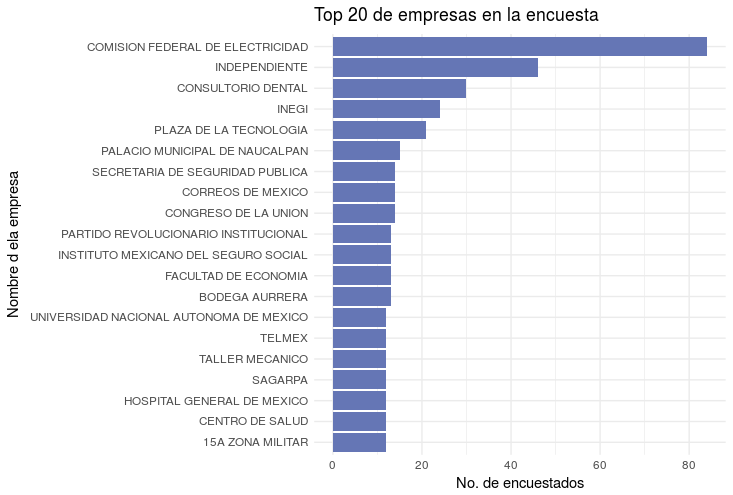
\includegraphics[scale=.5]{20_empresas.png}
    \caption{ Las 20 empresas con mayor participación en la encuesta. Mientras que la gran mayoría solo presenta una, las presentadas en la gráfica son las más de mayor presencia. Notese que en su mayoria son de iniciativa publica lo que podría estar sesgando la muestra. }
    \label{figura1_2}
  \end{center}
\end{figure}
En el cuestionario existe una pregunta abierta\footnote{Y capturada hasta en seis campos diferentes donde hay muchos datos faltantes.} sobre las actividades que realiza la empresa, su giro comercial o a grandes rasgos a lo que se dedica, esta parte fue contestada por el jefe en la primer fase de la entrevistas. La figura 1.3 muestra la respuesta de a qué actividades se dedica la empresa segun sus directivos o jefes inmediatos de los encuestados. 

\begin{figure}[H]
  \begin{center}
    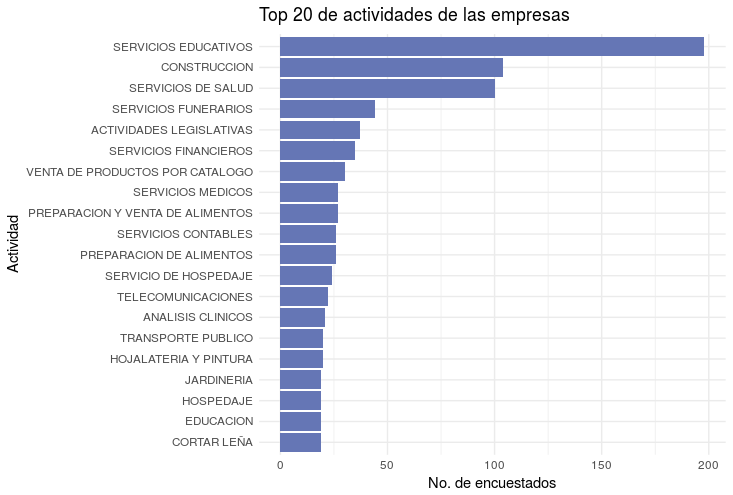
\includegraphics[scale=.5]{20_actividades.png}
    \caption{ Las 20 actividades con mayor participación en la encuesta. Notemos en este caso que las actividades ya no son cerradas a la iniciativa pública.}
    \label{figura1_2}
  \end{center}
\end{figure}

Para terminar con la descripción de la primer parte de las entrevistas, se tiene la figura 1.4 la cual muestra la distribución de las actividades económicas de las empresas en la muestra y finalmente la pregunta número 6 es: 
\textbf{En el último año ¿Cuáles fueron las principales vacantes requeridas por esta empresa, institución u organización?}, la cual es una pregunta puntual y que es bueno saber para que los futuros empleados de cierto grupo desarrollen esas habilidades, siguiendo uno de los objetivos de CONOCER.\\

La respuesta a esta pregunta se capturó en 7 campos de nuestro conjunto de datos, si bien un estudio de frecuencia de palabras suena atractivo eso no aprovecha la información que provee en concepto. Por lo que realizamos un conteo de frases que se presentan en la figura 1.5 donde en contra de nuestra intuición vemos que las habilidades más recurrentes, para el 2011 (año en que se aplicó la encuesta) fueron del tipo de habilidades blandas o soft skills en lugar de las habilidades técnicas. 

\begin{figure}[H]
  \begin{center}
    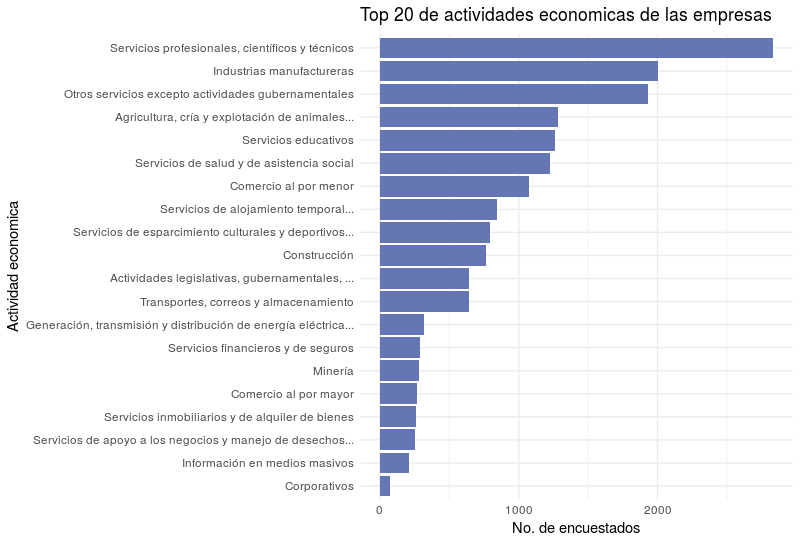
\includegraphics[scale=.5]{20actecon.png}
    \caption{ Las 20 actividades economicas con mayor participación en la encuesta.}
    \label{figura1_3}
  \end{center}
\end{figure}

\begin{figure}[H]
  \begin{center}
    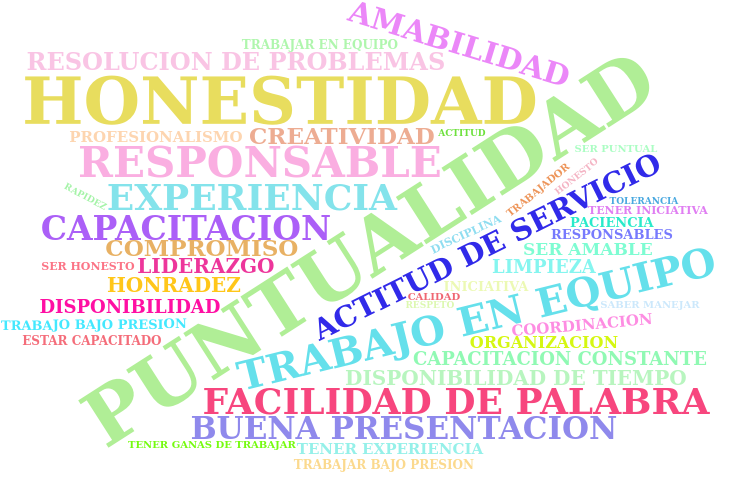
\includegraphics[scale=.4]{vacantes_requeridas.png}
    \caption{ El tamaño de la frase indica su frecuencia relativa con respecto del grupo de frases respuesta de la pregunta 6. Nótese que el trabajo en equipo es una de las más recurrentes.}
    \label{figura1_5}
  \end{center}
\end{figure}

Comentemos rápidamente la parte cualitativa de la segunda sección de la entrevista. En la figura 1.6 se encuentre otra nube de palabras pero ahora la información que refleja son los principales riesgos laborales en su puesto \footnote{Nuevamente esta pregunta es abierta y se registra en 6 columnas de nuestro conjunto de datos.} donde notamos que los riesgos laborales son los de la vida cotidiana (o por lo menos los más frecuentes de nuestra muestra), por otro lado la figura 1.7 muestra la frecuencia a la pregunta: \textbf{Si alguien fuera a ser contratado(a) para desempeñar este trabajo, desde su punto de vista, ¿cuánto tiempo de experiencia debería tener?} los resultados concuerdan con mi experiencia experiencia personal pues en general se piden de 1 a 4 años de experiencia para solicitar un empleo (sin embargo recordemos que las personas que respondieron a la encuesta tenían cuando menos un año en su posición) y la figura 1.8 muestra el nivel educativo que el encuestado considera apropiado para alguien desarrollando sus mismas actividades.
\begin{figure}[H]
  \begin{center}
    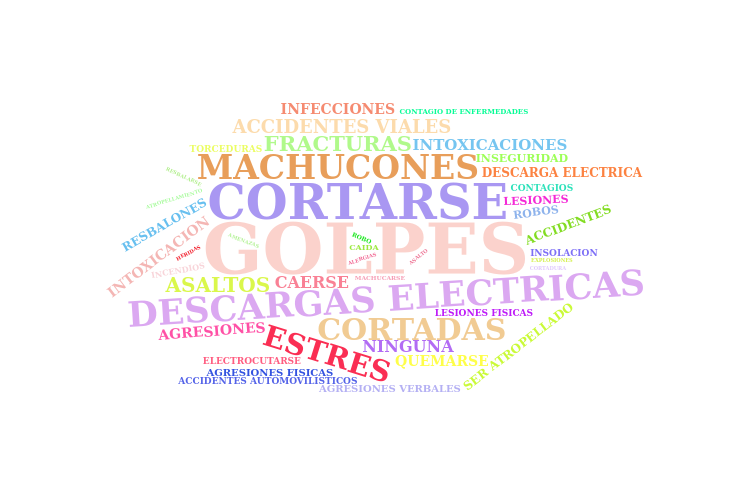
\includegraphics[scale=.5]{50_riesgos.png}
    \caption{ Los 50 riesgos más frecuentes en su zona de trabaja que considera la muestra encuestada}
    \label{figura1_6}
  \end{center}
\end{figure}

\begin{figure}[H]
  \begin{center}
    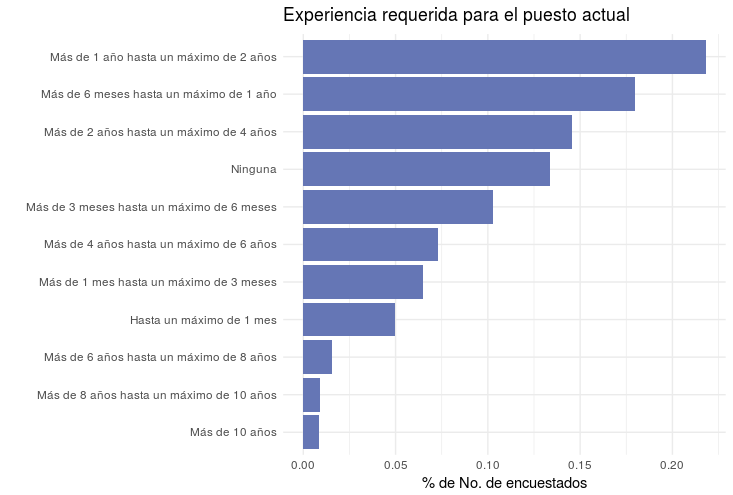
\includegraphics[scale=.5]{experiencia.png}
    \caption{Distribución de la experiencia requerida para ocupar su puesto (recordemos que esta respuesta está condicionada a quien la persona que contesta tiene más de un año de experiencia en el grupo de trabajo actual). }
    \label{figura1_7}
  \end{center}
\end{figure}
\FloatBarrier

\begin{figure}[H]
  \begin{center}
    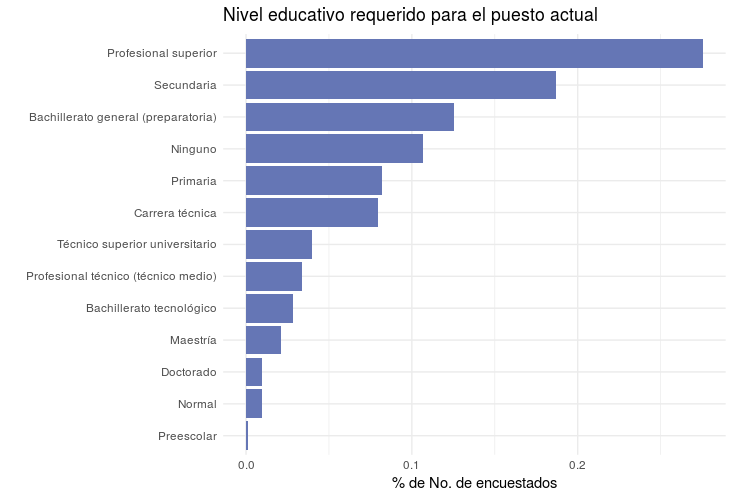
\includegraphics[scale=.5]{educacion.png}
    \caption{Nivel de estudios que un nuevo candidato debería tener para el mismo puesto según los entrevistados.}
    \label{figura1_8}
  \end{center}
\end{figure}
\FloatBarrier

En la siguiente sección continuamos con la metodología empleada, MDS unfolding para intentar encontrar relaciones entre los grupos (o bien ocupaciones) y las habilidades que se preguntan.





\section{Resultados}
En vista del cómputo con el que se cuenta, no fue factible realizar MDS unfolding considerando todas las 102 variables categóricas, por lo que los valores reportados por ellas se consideran continuos\footnote{Proponiendo para un trabajo futuro el mismo análisis pero considerando una técnica de clusterización y unfolding simultánea.}.\\

Con fines meramente de visualización en la figura 2.1 se muestra el resultado de aplicar MDS unfolding considerando solo dos dimensiones, recordemos que los grupos definen ocupaciones.


\begin{figure}[H]
  \begin{center}
    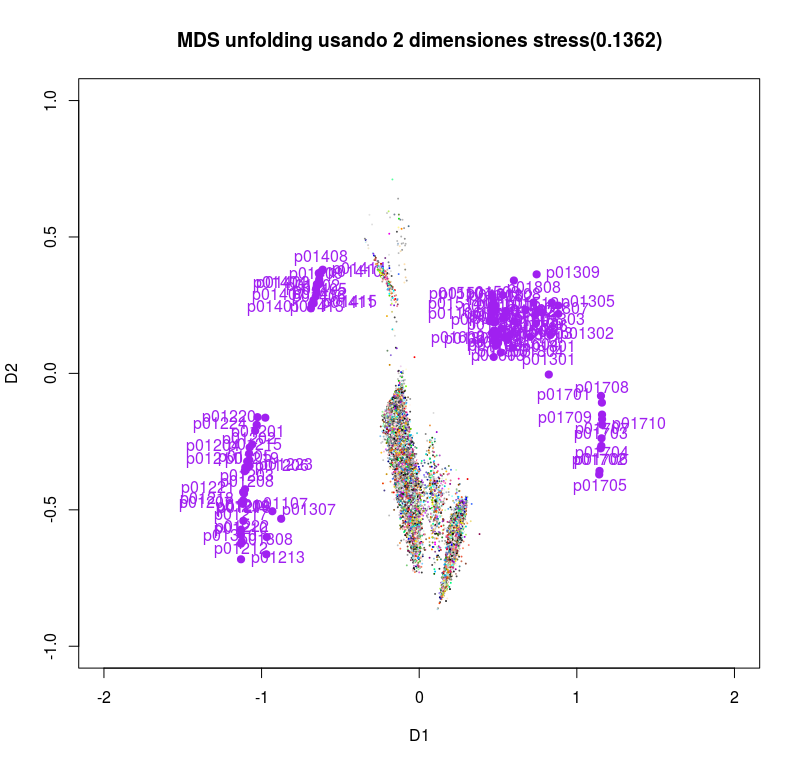
\includegraphics[scale=0.5]{2D.png}
    \caption{Resultado de aplicar MDS unfolding sobre todo nuestro conjunto de observaciones en el rango $[1,5]$ en 2 dimensiones. Los puntos morados son las columnas, los puntos de colores corresponden a entrevistados (donde el color determina su ocupación), notemos que es difícil de apreciar una agrupación entre las habilidades y las ocupaciones.}
    \label{figura4_2}
  \end{center}
\end{figure}

Para poder estimar el número apropiado de la dimensión con la cual emplear MDS unfolding, se realizaron dos simulaciones\footnote{Debido a las limitaciones en cómputo, además previamente se obtuvo una buena distinción usando 40 dimensiones.} cada una considero una muestra aleatoria de la mitad total y se obtuvo el stress adquirido para cada valor de dimensión en cada simulación. Los resultados se muestran en la figura 2.2 los cuales parecen indicar que la el número de dimensión para un buen ajuste de MDS unfolding es un parámetro estable.


\begin{figure}[H]
  \begin{center}
    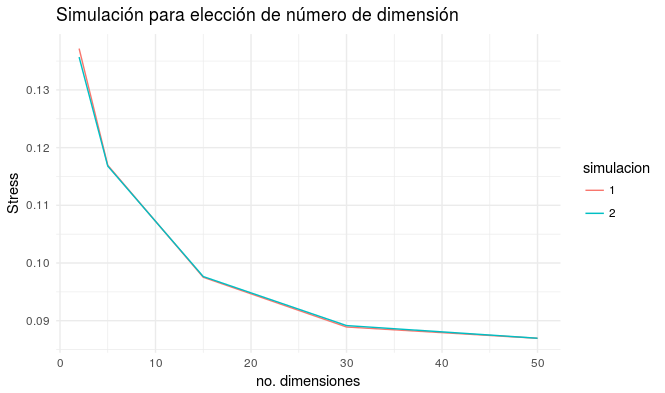
\includegraphics[scale=0.65]{dimension.png}
    \caption{Resultados de la realización de dos simulaciones, cada una considero una muestra aleatoria de la mitad total y se obtuvo el stress adquirido para cada valor de dimensión en el conjunto  $\{2,5,15,30,50\}$. Observando las curvas y usando el criterio del codo determinamos que un buen número para la dimensión a representar es 35 para la muestra total (considerando el error de nuestro submuestreo). }
    \label{figura2_2}
  \end{center}
\end{figure}

Con la información de la figura anterior y recordando que las simulaciones se realizaron solo con la mitad de tamaño de muestra se consideró finalmente un modelo MDS unfolding con 35 dimensiones. Los resultados se muestran en la figura 2.3 donde podemos apreciar que existen cuando menos 4 cluster de empleos, tres de ellos a su vez contienen diferentes tipos de grupos (indicado por el color de los puntos) lo cual es ad hoc con la construcción de esta agrupación que realiza el SINCO la cual consiste en 4 niveles jerárquicos. Notemos sin embargo que el pequeño grupo formado por los puntos negros se diferencia fácilmente y está cercano (en esta proyección) a las habilidades: razonamiento numérico, comunicación verbal y escrita, pensamiento analitico, capacidad de sintesis e información (con etiquetas en la gráfica p01401 hasta p01415).    
\begin{figure}[H]
  \begin{center}
    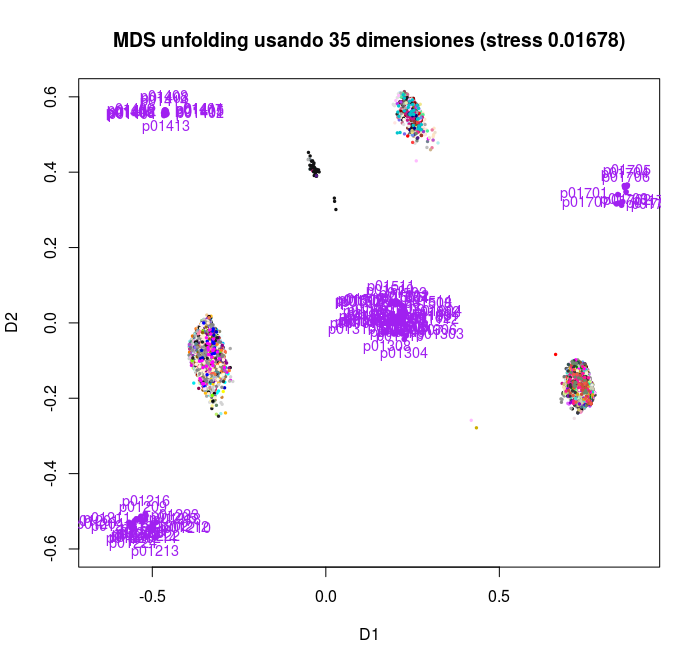
\includegraphics[scale=0.75]{35dimensiones.png}
    \caption{Resultado de aplicar MDS unfolding sobre todo nuestro conjunto de observaciones en el rango $[1,5]$ en 35 dimensiones. Los puntos morados son las columnas, los puntos de colores corresponden a entrevistados (donde el color determina su ocupación), notemos que no es difícil de apreciar 4 conjuntos de ocupaciones.}
    \label{figura2_3}
  \end{center}
\end{figure}
Existen elementos para afirmar que hay tres direcciones determinadas por las habilidades, las cercanas al origen de la anterior proyección las cuales corresponden al uso de maquinaria y diversas actitudes sociales parecen estar alineadas a las del grupo de habilidades localizadas en la imagen arriba derecha y que corresponden a destrezas como trabajar en oficina o con público, la segunda dirección localizadas en la parte superior izquierda las habilidades de tipo gerencial e intelectual (aparentemente ortogonales a las anteriores direcciones
) y finalmente la dirección determinada por las habilidades relacionadas al conocimiento de diferentes disciplinas (abajo izquierda).\\

Finalmente para validar los resultados obtenidos con MDS unfolding, los contrastamos con los resultados que se obtendrían usando PCA.\\


Para ello primero realizamos un estudio paralelo, como el planteado en \cite{Parallel}\footnote{Un trabajo muy interesante  donde se mencionan ciertos detalles de porque el criterio de Kaiser no siempre es adecuado, pues no considera errores de muestreo o de otras fuentes.}, para determinar el número de componente principales a utilizar, para ello realizamos 10 simulaciones, cada una de ellas construye una matriz con 102 columnas y 17250 filas con entradas en $\{1,2,...,5\}$ simuladas uniformemente en ese conjunto y asumimos independencia entre las variables, posteriormente se obtuvo su matriz de correlación y se obtuvieron los vectores propios correspondientes a todas las componentes principales. El resultado de la simulación se muestra en el figura 2.4 (arriba izquierda), al introducir la información (muestral) de los valores propios de la encuesta se nota la diferencia en sus magnitudes (imagen 2.4 arriba derecha) y la simulación parece indicar que 15 componentes principales serían un buen número de dimensiones para representar a nuestro conjunto de datos (imagen 2.4 abajo izquierda).

 

\begin{figure}[H]
  \begin{center}
    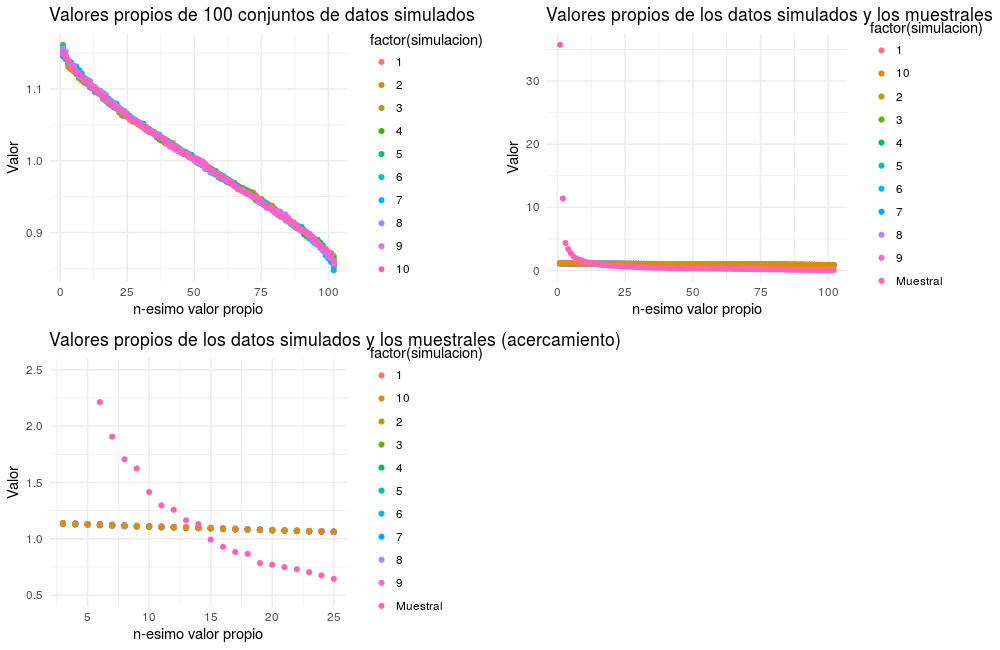
\includegraphics[scale=0.45]{pca_n.png}
    \caption{Análisis paralelo para determinar el número de componentes principales para representar las variables cuantitativas de la encuesta.}
    \label{figura2_4}
  \end{center}
\end{figure}


Sin embargo al realizar el cálculo necesario para obtener las componente principales con matriz de correlación obtenemos que la primer componente explica por si misma 87\% de la varianza total y la segunda aporta otro 5\%. Los resultados de las proyecciones de los individuos se muestran en la figura 2.5, donde nuevamente el color indica el grupo de ocupación. Notemos que en esta caso no se posible distinguir grupos claramente dos grupos.\\

Donde la primer componente principal tiene pesos mayores en las respuestas de las secciones 12,14 y 17 que son precisamente habilidades específicas como manejo de maquinaria o equipo de cómputo y la segunda componente tiene cargas considerables en todas las demás respuestas que conciernen a habilidades menos técnicas.

\begin{figure}[H]
  \begin{center}
    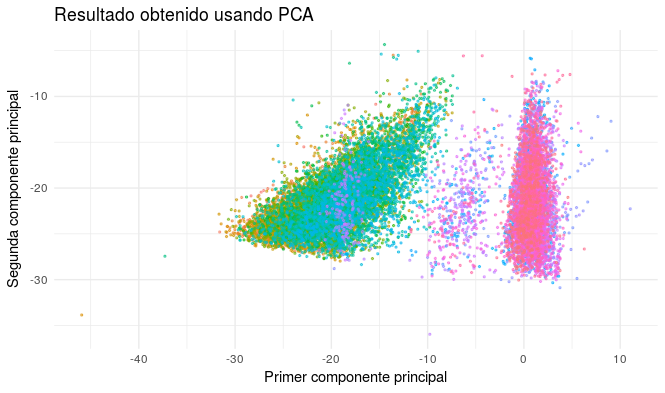
\includegraphics[scale=0.8]{resultado_pca.png}
    \caption{Proyección de los datos de la encuesta cuantitativos en sus dos primeras componentes principales usando matriz de correlación.   }
    \label{figura2_5}
  \end{center}
\end{figure}

\newpage
\section{Conclusiones}

El obetivo primario se cumplio parcialmente, pues pudimos determinar, por medio de MDS unfolding, que las habilidades de la encuesta determinan grupos entre ellas mismas y estas han sido presentadas de manera conjunta en la encuesta (hecho que se ve reflejado en que en la figura 2.3 se forman grupos con variaciones en sus últimos dígitos de etiquetas) sin embargo seguiríamos en mayor nivel de detalle o bien descartar algunas de las respuestas de las preguntas 13,15 y 16 pues no parecen medir impulsos diferentes en la muestra encuestada. Por otro lado las preguntas 12, 14 y 17 parecen ser fundamentales para tener diferenciadores en las diferentes habilidades. El punto en donde el objetivo primario no se logró a profundidad es que si bien se identificaron 4 grupos de ocupaciones finalmente no podríamos asignar a nivel grupo un conjunto de habilidades, esto se relaciona con nuestra conclusión del objetivo secundario el cual conlleva a dos ideas, identificar subgrupos en los grupos encontrados (como un trabajo futuro con mayor información e incluyendo como otro modo del MDS al sector económico como lo hizo el Dr. Miguel Flores) o bien en revisar la teoria estadistica de muestreo y diseño de experimentos para poder evaluar la calidad de los datos presentados porque quizá las condiciones y la forma (greedy para aminorar costos) no fue la mejor decisión, para afinar y mejorar el diseño de la encuesta.

En este sentido se concluye y reitera la ide del Dr. Miguel Flores han pasado ya 7 años desde la aplicación de esta encuesta y una implementación digital utilizando tecnologías accesibles e inclusive opensource (como la mencionada anteriormente Shiny y la infraestructura del ambiente R) podrían abaratar el precio de actualizar la encuesta y llegar a un mayor número de grupos, industrias y analizar en tiempo real los datos y los resultados. Lo cual también plantea un posible trabajo futuro de cómputo estadístico pues los métodos empleados en este análisis son computacionalmente intensivos.

 



\newpage

\begin{thebibliography}{1}

\bibitem{Parallel}
Horn, J.L. \emph{A rationale and test for the number of factors in factor analysis
}, Psychometrika (1965) 30: 179. \url{https://doi.org/10.1007/BF02289447}

\bibitem{roris}
Ingwer Borg, Patrick J.F. Groenen (2005), \emph{Modern Multidimensional Scaling}, Springer, 2da edición. 

\bibitem{smacof}
Jan de Leeuw, Patrick Mair (2009). \emph{Multidimensional Scaling Using Majorization: SMACOF in R}, Journal of Statistical Software, 31(3), 1-30. \url{http://www.jstatsoft.org/v31/i03/}

\bibitem{Rsmacof}
Jan de Leeuw and Patrick Mair, \emph{Multidimensional Scaling Using Majorization: SMACOF in R}, versión 1.10,\url{https://cran.r-project.org/web/packages/smacof/index.html}


\bibitem{R}
R Core Team, \emph{R: A Language and Environment for Statistical Computing}, R Foundation for Statistical Computing; Vienna, Austria, 2014 y  \url{http://www.R-project.org/}


\bibitem{Shinydashboard}
Winston Chang and Barbara Borges Ribeiro (2018),\emph{shinydashboard: Create Dashboards with 'Shiny'}, R package version 0.7.0, \url{https://CRAN.R-project.org/package=shinydashboard}





\end{thebibliography}

\end{document}